\section{Experiments}
\label{experiments}

\subsection{Synthetic data}

We consider three differents latent-variable Gaussian graphical models.

The first model consists of $p=90$ observed variables and $h=3$ latent variables, we split observed variables in three groups of size $30$ and connect each group to a single latent variable. The second model is formed by $p=30+15+5=50$ observed variables and $h=3$ latents variables we split observed variables in three groups of different sizes ($30,15$ and $5$) and connect each group to a single latent variable. The third model consists of $p=$ observed variables and $h=5$, we select $5$ overlapping groups of observed variables, with an overlap of $ $, and connect each one of them to a different latent variable.

For all three models the conditional graphical model structure of the observed variables is a tree with the edge partial correlation coefficients equal to 0.25. 

k-3-blocs+tree structure\\

different size blocs\\

overlapping blocs\\

%\begin{figure}[h]
%  \begin{minipage}[ccc]{\linewidth}
%  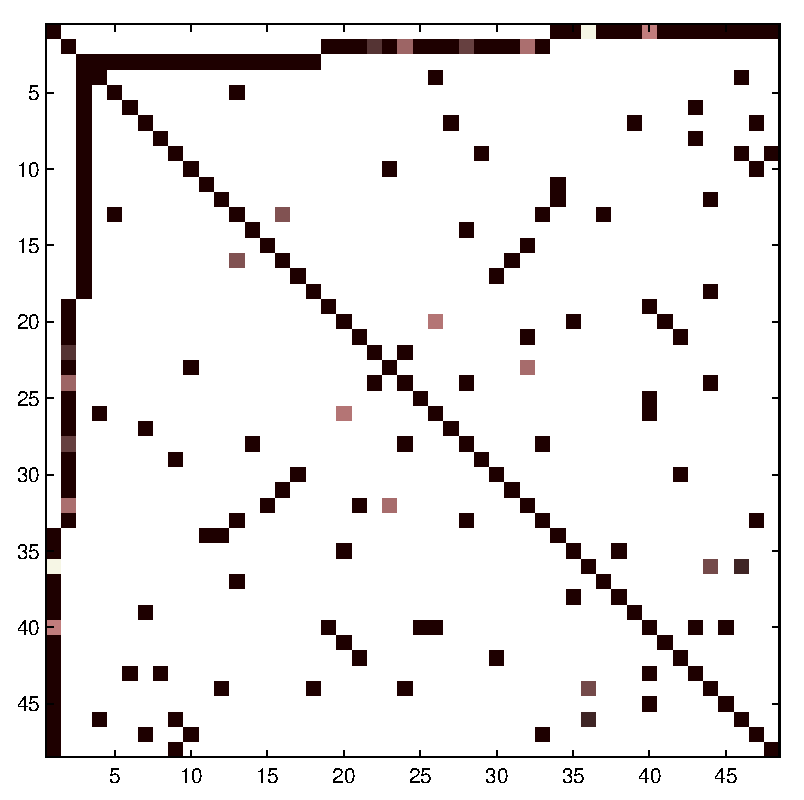
\includegraphics[width=3cm]{fig/disjoint_om}
%  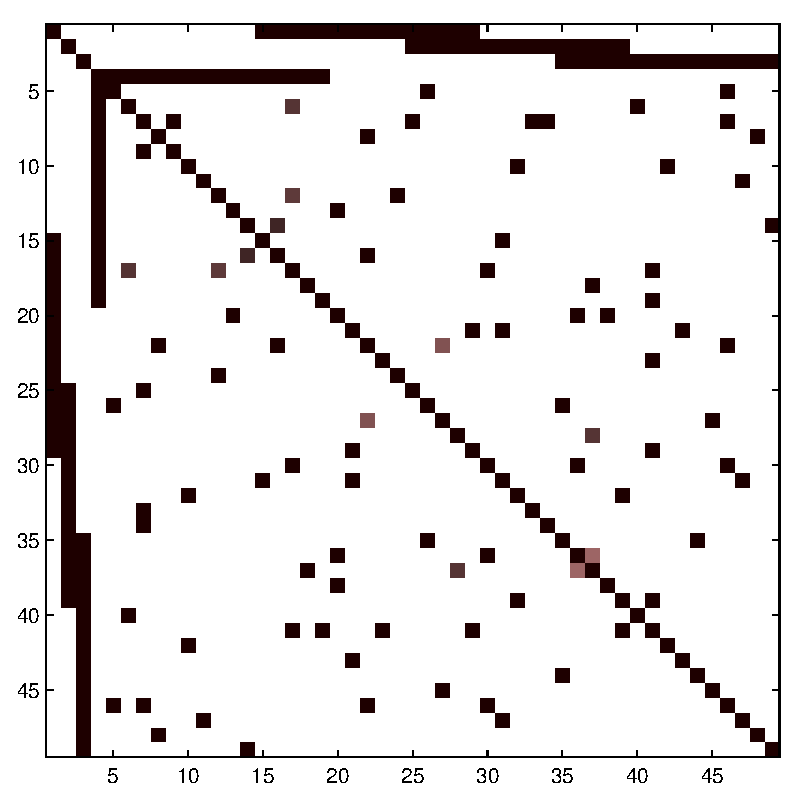
\includegraphics[width=3cm]{fig/overlap_om}
%  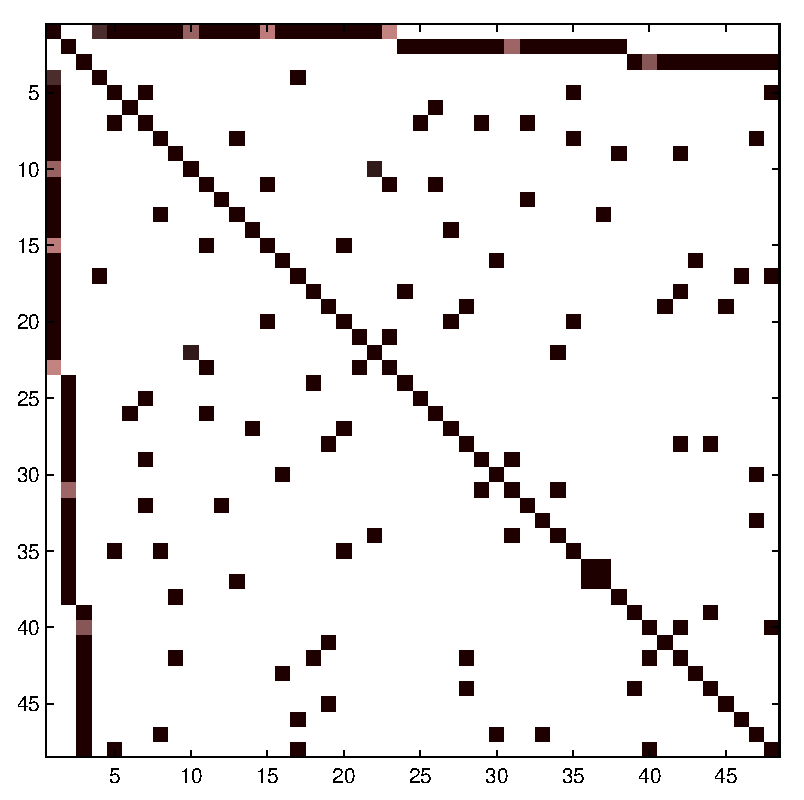
\includegraphics[width=3cm]{fig/diff_om}
%  \end{minipage}
%  \begin{minipage}[ccc]{\linewidth}
%  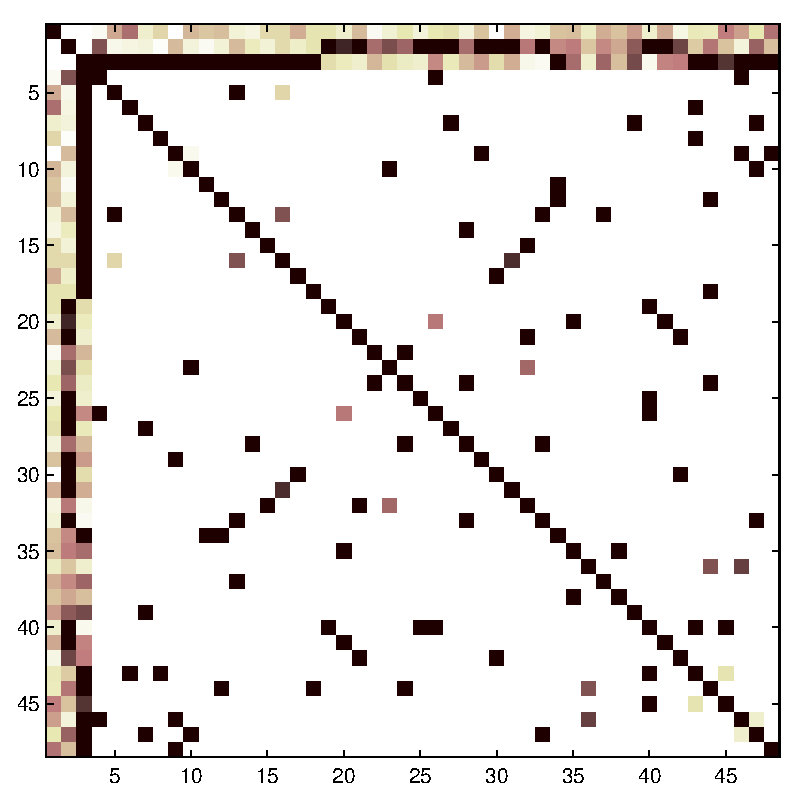
\includegraphics[width=3cm]{fig/disjoint_tr}
%  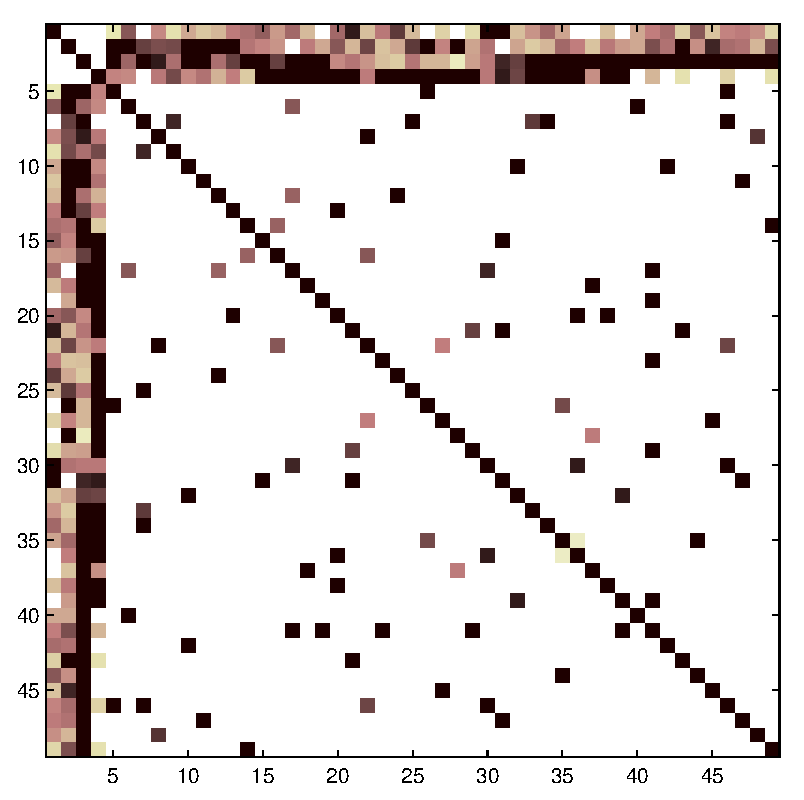
\includegraphics[width=3cm]{fig/overlap_tr}
%  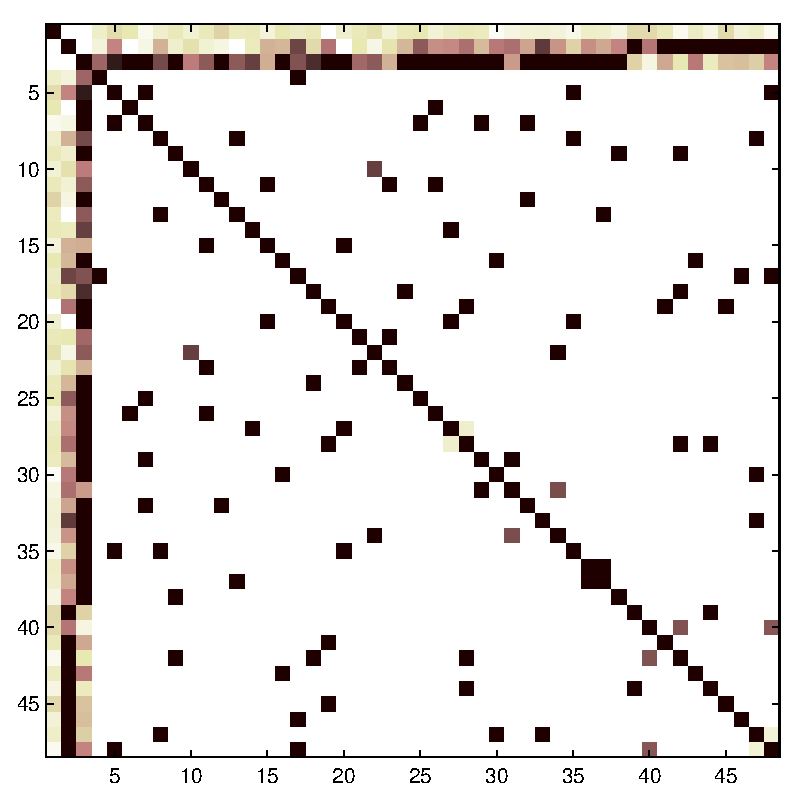
\includegraphics[width=3cm]{fig/diff_tr}
%  \end{minipage}
%  \caption{Experiment for the $k$-chain group Lasso. Top:number of pivots, i.e., drop/full step in active set. Left figure shows the number of pivots per active set call and right plot shows the total number of pivots during iterations. Bottom: evolution of the number of active atoms in our algorithm.}
%\end{figure}

%\begin{figure}
%\center
%\hfill
%\subfigure[Title A]{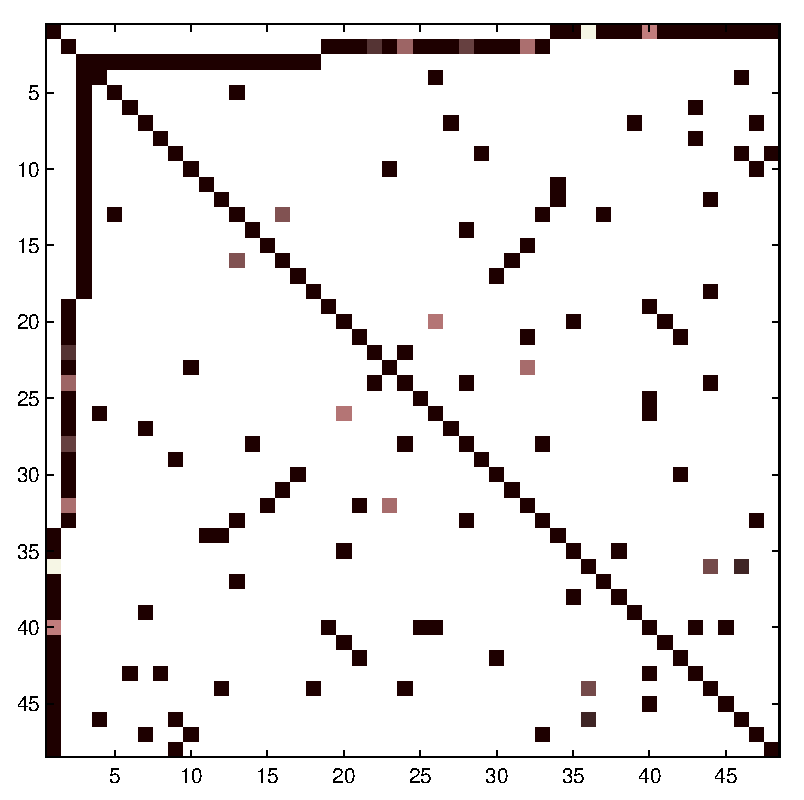
\includegraphics[width=3cm]{fig/disjoint_om}}
%\hfill
%\subfigure[Title B]{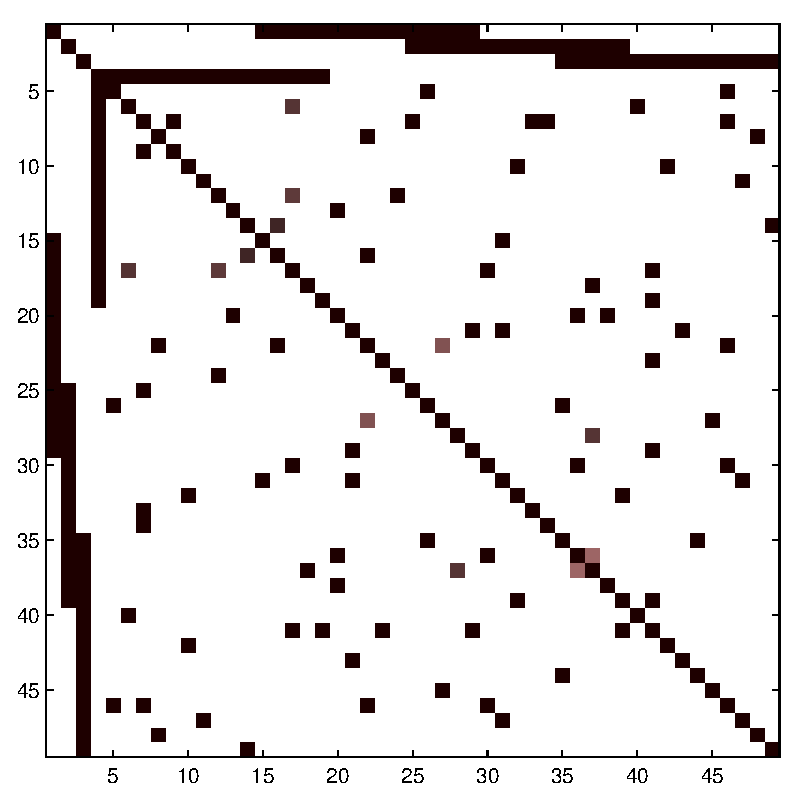
\includegraphics[width=3cm]{fig/overlap_om}}
%\hfill
%\subfigure[Title C]{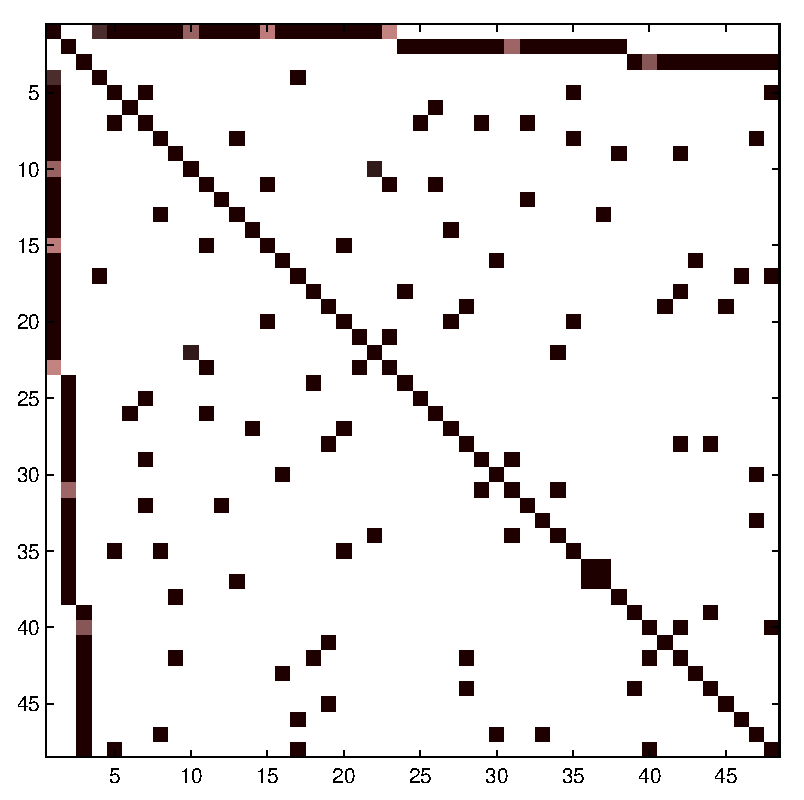
\includegraphics[width=3cm]{fig/diff_om}}
%\hfill
%\\
%\subfigure[Title A]{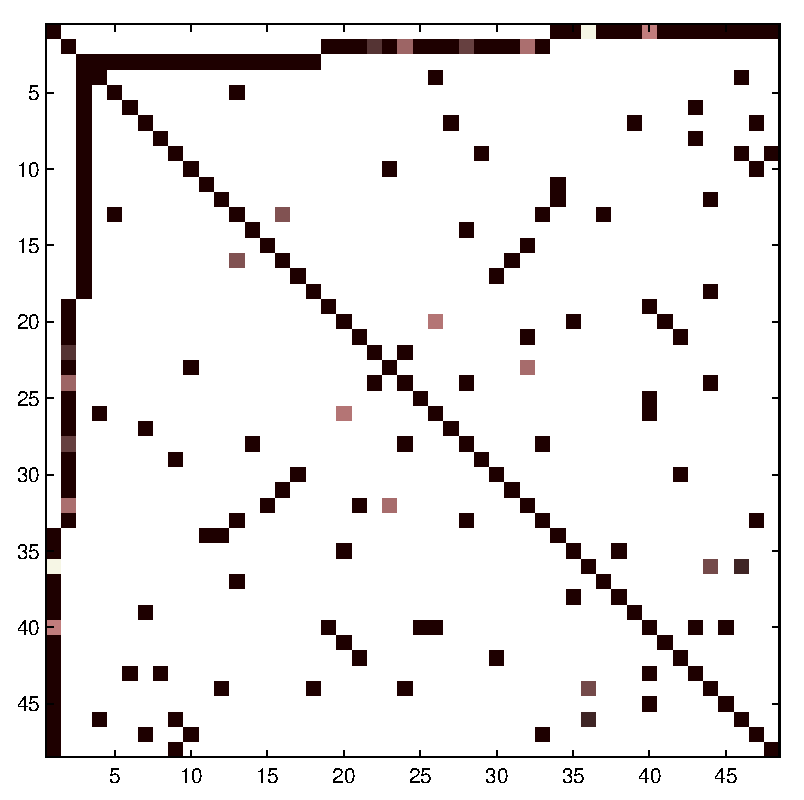
\includegraphics[width=3cm]{fig/disjoint_om}}
%\hfill
%\subfigure[Title B]{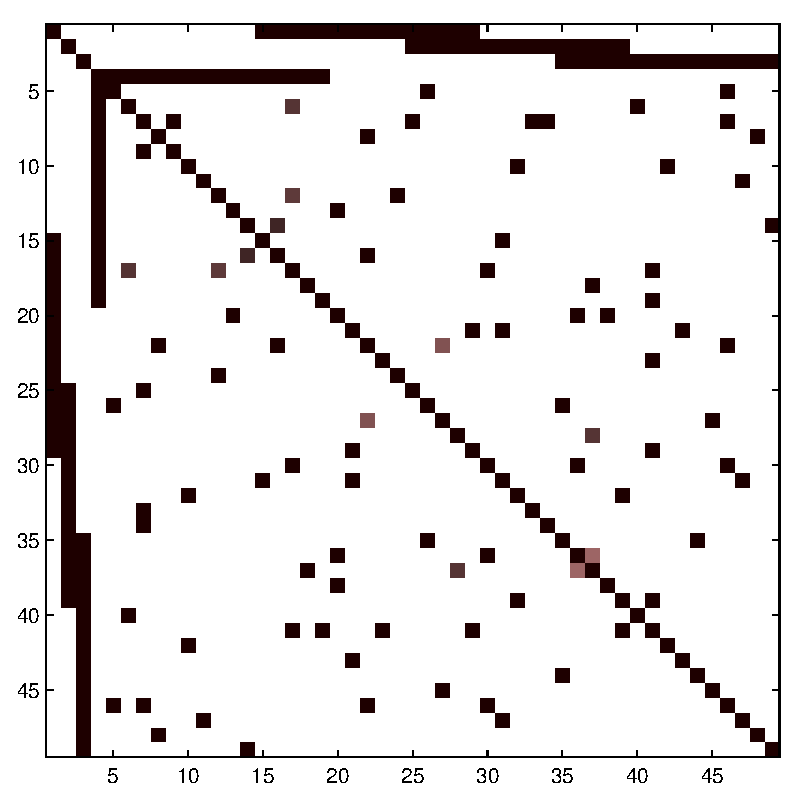
\includegraphics[width=3cm]{fig/overlap_om}}
%\hfill
%\subfigure[Title C]{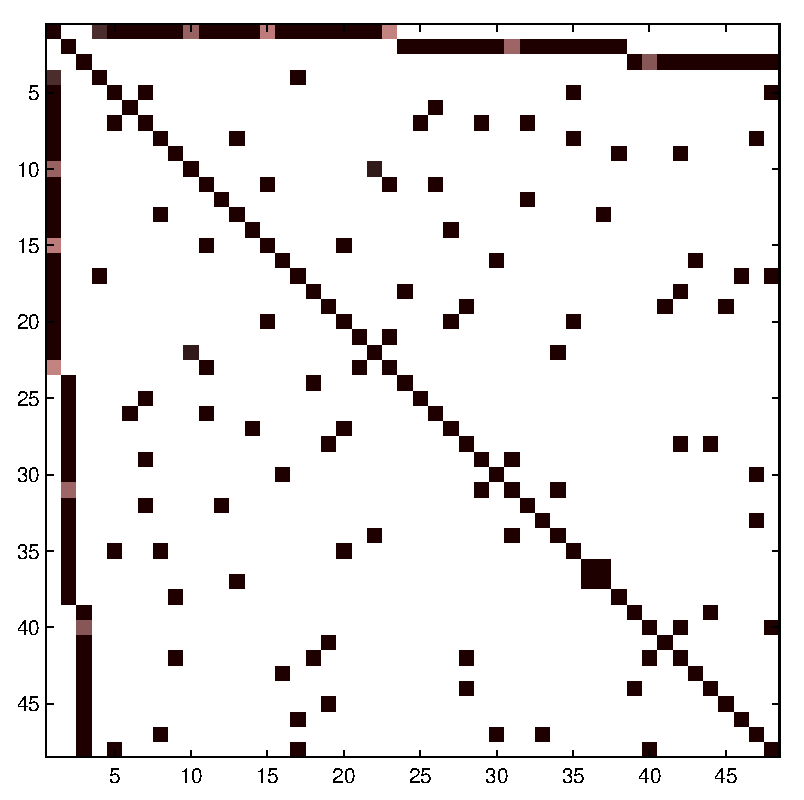
\includegraphics[width=3cm]{fig/diff_om}}
%\hfill
%\caption{Title for both}
%\end{figure}

\begin{figure}
\center
\hfill
\subfigure[Title A]{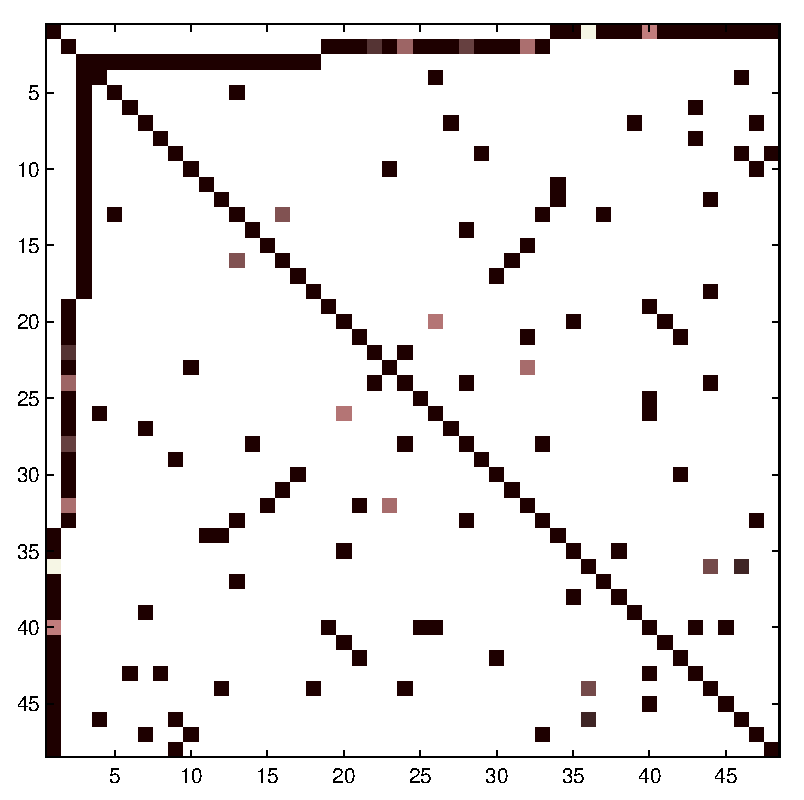
\includegraphics[width=2.2cm]{fig/disjoint_om}}
\hfill
\subfigure[Title B]{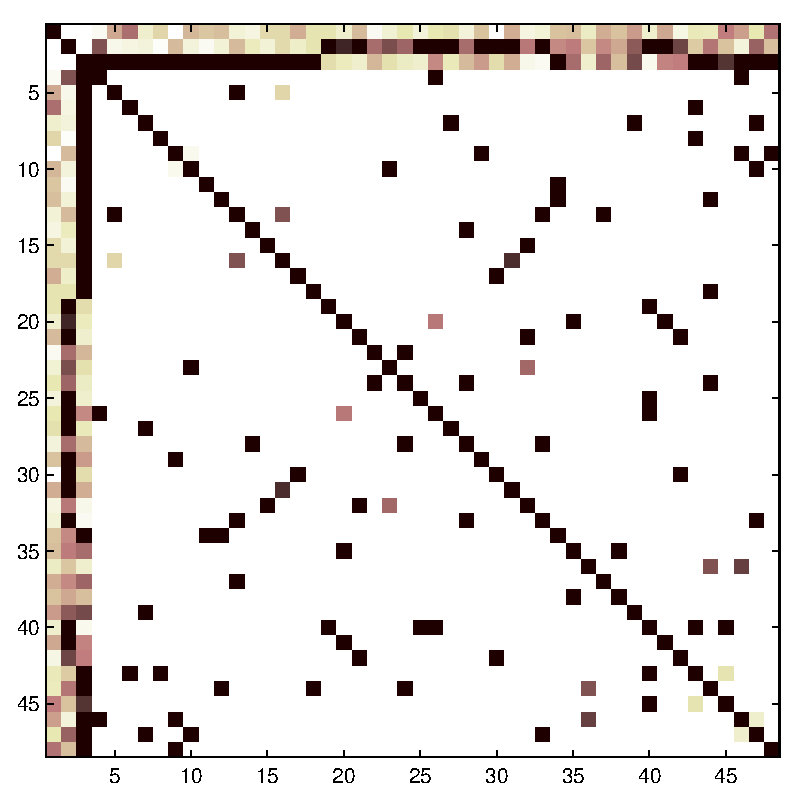
\includegraphics[width=2.2cm]{fig/disjoint_tr}}
\hfill
\subfigure[Title C]{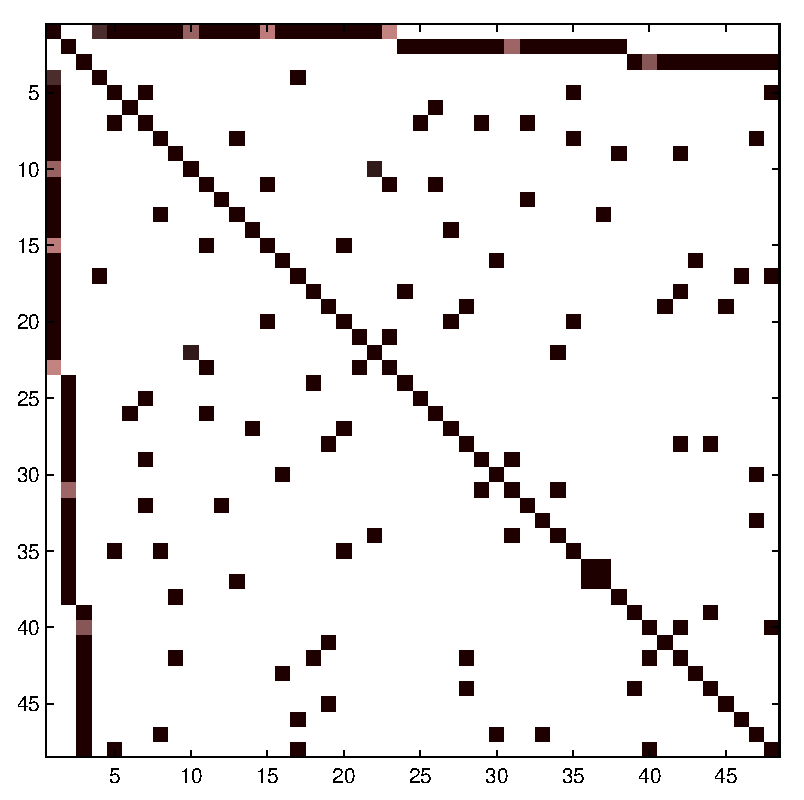
\includegraphics[width=2.2cm]{fig/diff_om}}
\hfill
\subfigure[Title A]{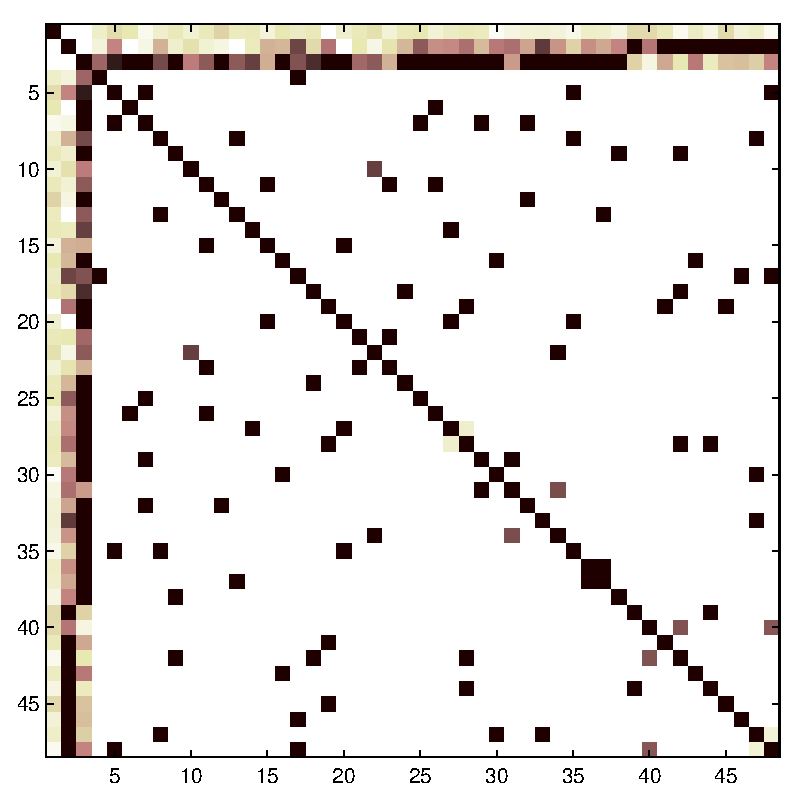
\includegraphics[width=2.2cm]{fig/diff_tr}}
\hfill
\subfigure[Title B]{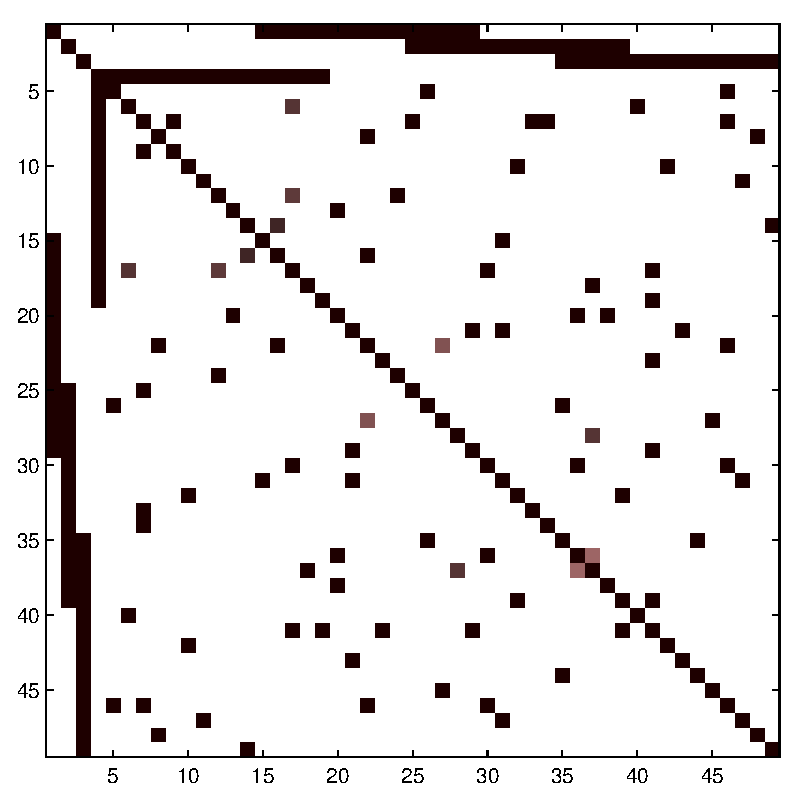
\includegraphics[width=2.2cm]{fig/overlap_om}}
\hfill
\subfigure[Title C]{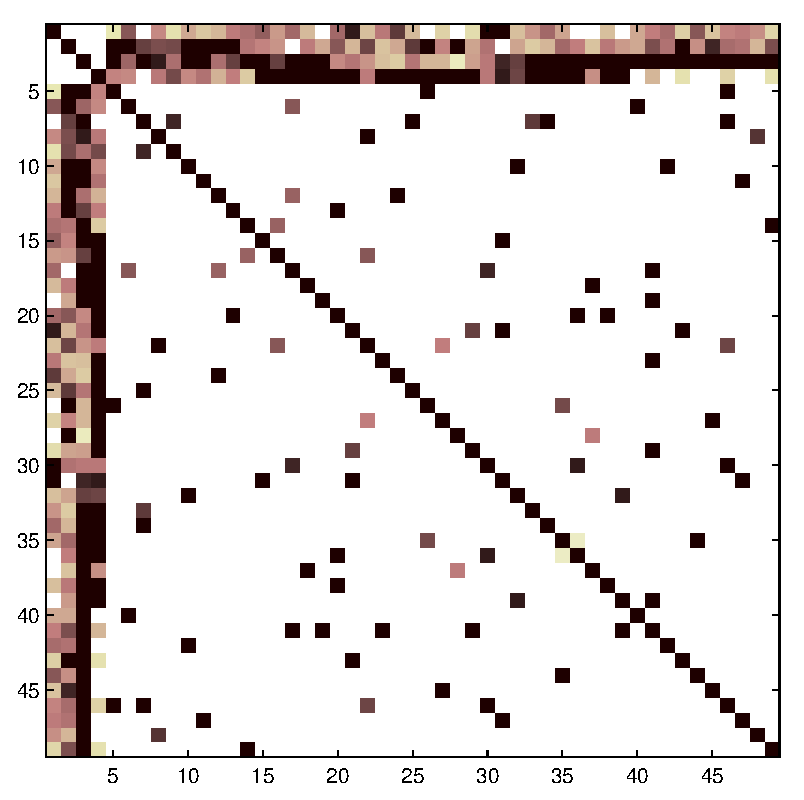
\includegraphics[width=2.2cm]{fig/overlap_tr}}
\hfill
\caption{Title for both}
\end{figure}


\subsection{dataset}